

\chapter{实施与维护} % Introduction chapter suppressed from the table of contents

\hypertarget{ux51c6ux5907ux8fedux4ee3ux56deux987e-qa}{%
\subsection{准备迭代回顾
Q\&A}\label{ux51c6ux5907ux8fedux4ee3ux56deux987e-qa}}

两个月前,为北京某企业做差距分析,发现大量缺陷在系统测试才被发现,建议加强迭代回顾根因分析。质量经理便开始尝试内部推动,并在两周前做了一次团队回顾辅导。

\hypertarget{ux505aux597dux73b0ux573aux8f85ux5bfc}{%
\subsubsection{做好现场辅导}\label{ux505aux597dux73b0ux573aux8f85ux5bfc}}

质量经理:我们计划下周三就会与另一项目组做迭代回顾,他们团队共7-8人,2周前与另一团队使用便利贴做根因分析,确实能听到更多不同的声音。应如何准备好,让今次这团队能放开并做好根因分析?\\
我:让我分享一下我的相关经验:\\

\framebox{%
\begin{minipage}[t]{0.97\columnwidth}\raggedright
如果他们没有学过根因分析,应先用15分钟介绍根因分析的主要元素(可用绅士俱乐部案例),然后立马请他们分两组,使用机场延误数据做45分钟互动练习。
(因利用数据,动脑筋,是最佳学习方式。因大家都坐过飞机,也遇过延误,应能理解机场的大概情况,所以不需要用实际团队缺陷数据。)

练习过程中,我只会定时提醒时间(需要在45分钟后跟管理层汇报),有时候在做练习时,学生会问我,''我做对不对啊?是否做错?``除非他们犯了基础错误(例如,用电脑打帕里托图,或只是按延误数据被一条按数字从最大排到最少等错误),我不会说你应该怎么做,尽量让团队自己讨论分析。团队都做完汇报以后,我才总结有哪些误解,那些做得好。
要做好回顾,准备很重要,例如要用大白纸,要有足够空间。如果团队成员都是围着一个大桌,坐下来讨论,不会有好结果。但反过来,如果我们在墙上贴上大白纸(1.5米
x
3米),并提供便利贴,大号、小号水笔,每个人有自己水笔写的时候,他们就会一直在走动,讨论,写字,画图,并不断交换位置,互相帮忙,这样就更能体现他们的团队意识更投入。

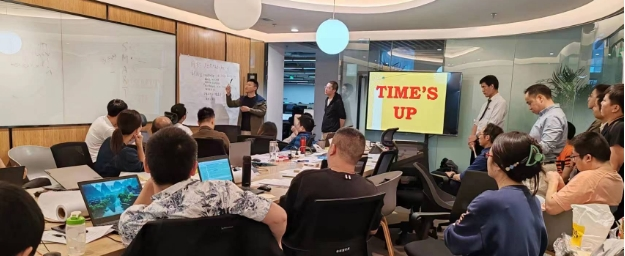
\includegraphics[width=6cm]{131.jpg}

\begin{description}
\tightlist
\item[]
(时间管理很重要。电脑投屏显示每轮活动剩下的时间(分钟),让团队即时知道还有多少时间。例如最后时间到会显示
"TIME'S UP")
\end{description}

机场飞机延误练习有几个很重要的特点:

\begin{itemize}
\tightlist
\item
  真实的数据让团队可以按练习依据数据去分析根因,而不是纯粹头脑风暴,定性分析。
\item
  有明确的任务目标(45分钟后给机场管理层汇报),给团队时间压力,团队便更有动力。只要任务明确,团队人员通常都有足够能力管理好自己分工,完成目标。
\end{itemize}

所以导师的任务不是教他一步一步怎么做,只要提醒时间,先定好目标,让他们团队自己发挥,自己讨论效果会更好。只要他们清楚需要做什么,大部分团队都能自己分好工,例如有些人画帕累托图,有些人做总体根因分析,或画鱼骨图,他们整个团队可能有五到八个人,我们作为导师就不需要帮他预先分工,他们自己会讨论自己会做好分工更好,尤其是已经是熟悉的、合作过的团队。

\strut
\end{minipage}}
质量经理:你的意思是要减少干预,尽量让团队自己动脑筋。但因未做过,可否再举些例子?\\
我:不如我反过来,建议你作为导师应该避免说什么:

\begin{enumerate}
\tightlist
\item
  其实你们团队我见到的其他团队好或者差(因这都是个人观点、感觉,非事实)。
\item
  本来只需要你们画帕累托图和鱼骨图,为什么你们还画了个脑图?
\item
  你们都已经讨论了很多细节,要立马赶紧时间做最后总结。
\item
  你们讨论好像都只是针对机场闸口的问题,是否应该也考虑其它?
\end{enumerate}

\framebox{%
\begin{minipage}[t]{0.97\columnwidth}\raggedright
为什么要鼓励团队表达不同意见?

如果团队要改进,首先应让大家充分理解各成员的差异,充分讨论后大家便应能自己找出共通点,才有机会一起改进。
\strut
\end{minipage}}


如果大家可以在回顾时开放讨论,把自己的具体看法说出来,就可以让大家看到全貌,真正的情况。

所以内部教练尽量要鼓励不同的声音发出来,ASCH
1951``从众实验''证明,只要有一位战友,团队成员就愿意表达自己意见.所以内部顾问尽量要让每个人都有充分机会发声,越多不同的意见提出来,大家越能了解真正的情况,找出一个大家都赞同的改进方案。(详见附件:功能性分组帮助团队成长实例)

例如,如果发现团队一起开大会,
因人多,不愿意发言,可能要分成小组讨论,效果更好。

有些团队比较``慢热'',便需要给他们多点时间,不怕沉默,等一下.只要等到有第一个人开始发言,后面就好办理了。

\hypertarget{ux5206ux6790ux5168ux8fc7ux7a0b}{%
\subsubsection{分析全过程}\label{ux5206ux6790ux5168ux8fc7ux7a0b}}

质量经理:好的,你说我们上次做了回顾还没有找到真正根因,但不知道如何改善。\\
我:可考虑分析流程。\\
某家电力服务公司的内部软件开发团队,公司规定每两周固定日期发新版,因客户对软件质量要求很高,每次都必须通过一系列的评审和测试才可以发版。\\
如果不能按发版时间完成项目交付,经理和团队会复盘整个过程,以识别在整个过程里哪些地方出现了失效点,然后针对失效点分析根因。所以除了模型,流程图也可以帮助分析过程并找出根因。画了流程图后,便可以利用FMEA方法针对每个失效点,找根因,和对应纠正措施。(详见附件``FMEA
实例'')

\framebox{%
\begin{minipage}[t]{0.97\columnwidth}\raggedright
某家公司专门为电信供应商做客服管理软件系统,因客户对质量有要求,每次发布后都分析有哪些发版后的问题。有些软件开发相关问题不容易排查根因,例如某次发布后发现报表的数字对不上,但这些错误不是立马使用时就出现,开始的时候没问题但使用时间长了,就会产生错误。

团队花了很长时间分析整个过程,最终发现错误是由于有些内部接口,没有考虑到所有传输数据是否正常,有些有错但没拒收,导致开始时没问题,但累积多了就会出现最后的报表错误。最后也针对这问题改正了。

讨论分析如何能避免同类问题:

%\href{文件:微信截图_20230928135611.png}{500px}
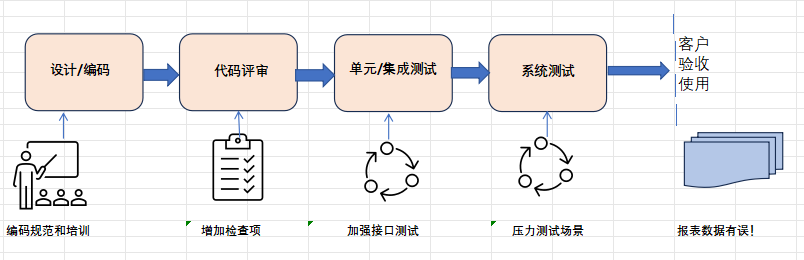
\includegraphics[width=6cm]{微信截图_20230928135611.png}


如果按系统产品集成的流程,识别有那些点可避免问题发生(FMEA思路)。可以在集成测试时和系统测试时,增加类似的场景,加大类似的压力测试,应可预先暴露问题;集成测试时,如果都测试所有接口传输的数据,也可以避免问题;如果我们前面做好设计和代码的评审(根源与设计有关),也应该可以避免。例如如果针对这种问题,完善评审检查单的检查项,以后应可避免同类问题再发生。
\strut
\end{minipage}}

所以从这实例可以看到针对技术问题,我们可以先画出从总体流程/路线图,每一个环节有什么风险,就可以更好的帮我们挖掘根因。

质量经理:你说我们上次缺乏具体量化目标,应如何改善?\\
我:用水晶球预测模型可以帮团队制定缺陷范围目标:\\

\hypertarget{ux56e2ux961fux7b2cux4e00ux8f6eux56deux987eux5b9eux4f8b}{%
\subsubsection{团队第一轮回顾实例}\label{ux56e2ux961fux7b2cux4e00ux8f6eux56deux987eux5b9eux4f8b}}

\begin{itemize}
\tightlist
\item
  团队分析迭代缺陷数据,缺陷是源自需求/设计/编码,得出以下分布表:
\end{itemize}

%\url{文件:微信截图_20220316093044.jpg}
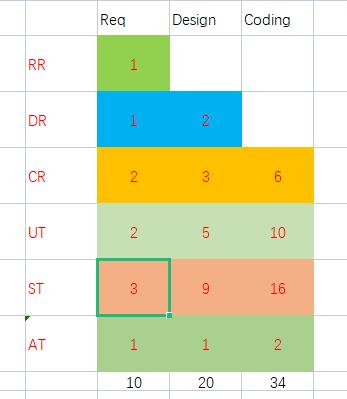
\includegraphics[width=6cm]{微信截图_20220316093044.jpg}

\begin{itemize}
\tightlist
\item
  按DRE公式,计算出各个过程的缺陷排除率
\end{itemize}

%\href{文件:2DreEstimateScreenshot_2021-12-01_212049.1.jpg}{文件:2DreEstimateScreenshot
%2021-12-01 212049.1.jpg}\\

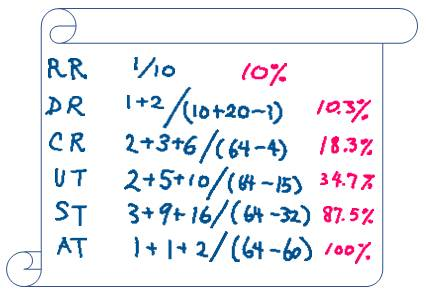
\includegraphics[width=6cm]{2DreEstimateScreenshot_2021-12-01_2120491.jpg}

\includegraphics[width=6cm]{sjb1.PNG}


%\href{文件:4reworkByPhaseScreenshot_2021-12-01_214838.1.jpg}{450px}


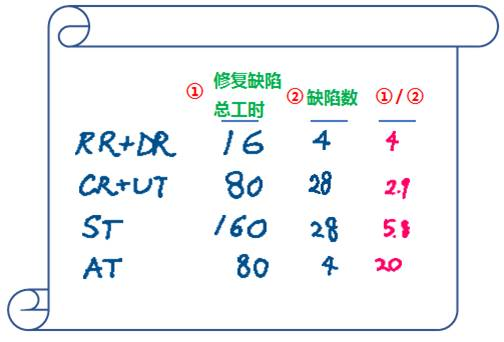
\includegraphics[width=6cm]{4reworkByPhaseScreenshot_2021-12-01_2148381.jpg}

\begin{itemize}
\tightlist
\item
  从团队工时表估算各过程的缺陷返工工作量。例如 最下面一行Quality
  那行输入:\$20,000 (因为验收测试缺陷平均修复工时是20,假定每工时成本为
  \$1,000);系统测试那行:\$5,800(因为系统测试缺陷平均修复工时是5.8)。
\end{itemize}

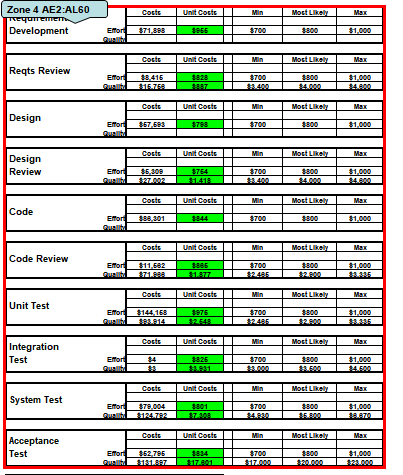
\includegraphics[width=6cm]{微信截图_20231031153355.png}

\begin{itemize}
\tightlist
\item
  估算质量总成本:水晶球会依据质每过程的缺陷分布和单位成本分布,预估质量成本的分布。按本来迭代需求引入缺陷数=10(3),需求评审缺陷排除率等于10\%(4),设计引入缺陷数=20(2),设计评审排除率=10\%(4),代码引入缺陷书=34(4),代码评审排除率=18\%(1),单元测试缺陷排除率=35\%(2),系统测试缺陷排除率=88\%(1),验收测试缺陷排除率=99\%(3)来估算质量成本分布。结果如下:(括号里的数字代表在模型参数表里那一栋,从1至4。)
\end{itemize}

%\href{文件:2AxtalBallPredictScreenshot_2021-12-01_212455.1.jpg}{400px}\\

%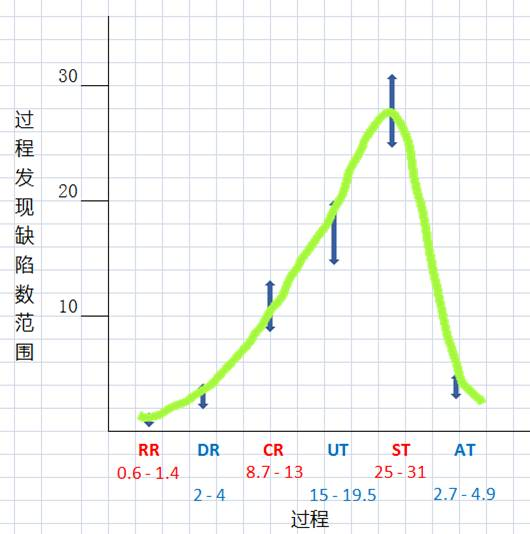
\includegraphics[width=6cm]{2AxtalBallPredictScreenshot_2021-12-01_2124551.jpg}

\includegraphics[width=6cm]{startQUA95.PNG}

从上图看到质量成本的分布, P95 (90\% percentile) = \$373,024

\begin{itemize}
\tightlist
\item
  团队经过根因分析找出纠正措施包括:

  \begin{itemize}
  \tightlist
  \item
    完善需求评审检查单,估计可以把评审缺陷排除率从10\%提升到80\%,但因为要完善检查单评审工时也会从本来的23人时增加到40人时。
  \item
    使用审查方式评审后台设计,估计可以把设计评审缺陷排除率从10\%提升到69\%,但评审工作量也会从48人时增加到65人时。
  \item
    使用代码走查方式,估计可以把代码评审缺陷排除率从18\%提升到35\%,但评审工作量也会从12人时增加到20人时。
  \end{itemize}
\end{itemize}

利用水晶球模型比较以上各种不同的配搭,选出总成本最低是配搭组合。在水晶球参数输入表格,在需求评审、设计评审和代码评审都加上新方法的工时和质量,在模型选最优配置需求评审可选方法(3、4)设计评审方法可选(3、4)代码评审可选方式(1、2)让模型从2
x 2 x 2 = 8种可选搭配中比较,挑选哪个搭配的总成本最低。

下图显示一直水晶球优化的过程,和最终的最``佳''配搭:

%\url{文件:微信截图_20211207132712.1.jpg}

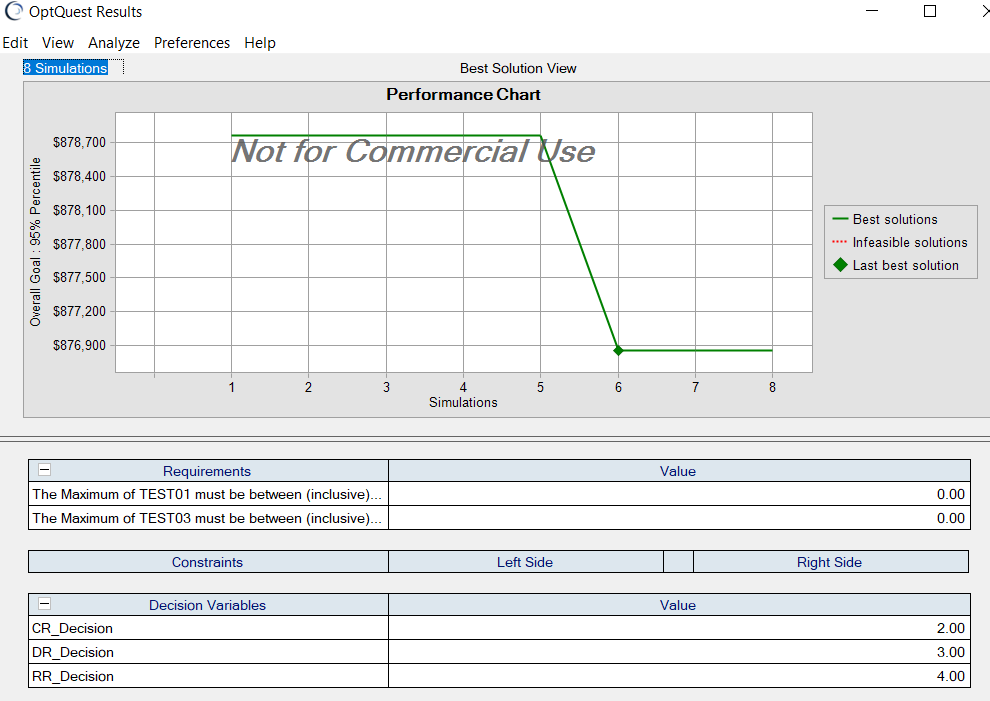
\includegraphics[width=6cm]{YH.PNG}

从上图看到最佳搭配是:

\begin{itemize}
\tightlist
\item
  代码评审(2)采用走查方式。
\item
  设计评审(3)采用审查方式。
\item
  需求评审(4)不变。
\end{itemize}

预测模型也会展示总成本的分布如下:

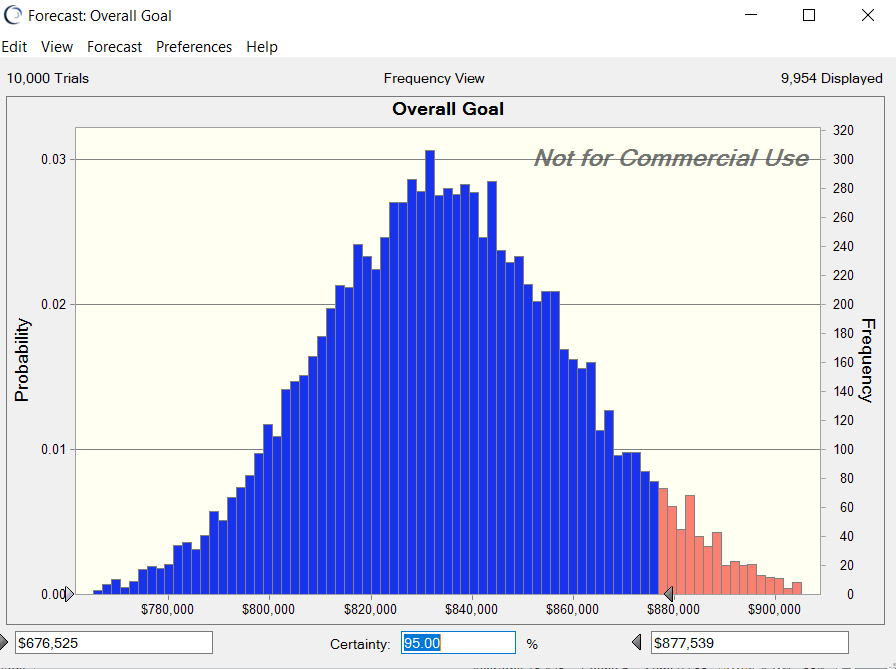
\includegraphics[width=6cm]{YH-OG95.PNG}

\begin{itemize}
\tightlist
\item
  预测模型依据我们输入的缺陷参数,得出每个过程的缺陷范围,例如系统测试缺陷数95\%
  上下限范围是15.2 至 19.1。例如单元测试缺陷数95\% 上下限范围是9.1至11.9。
\end{itemize}

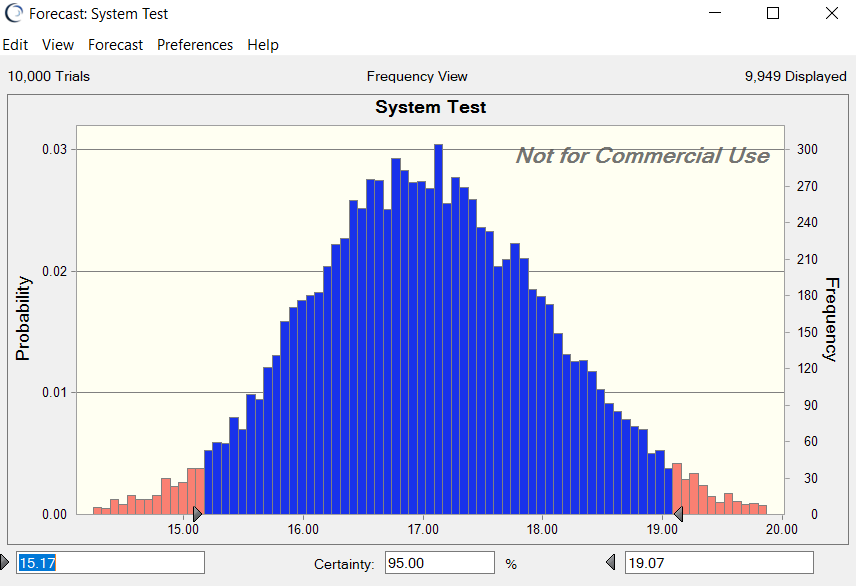
\includegraphics[width=6cm]{YH-ST.PNG}

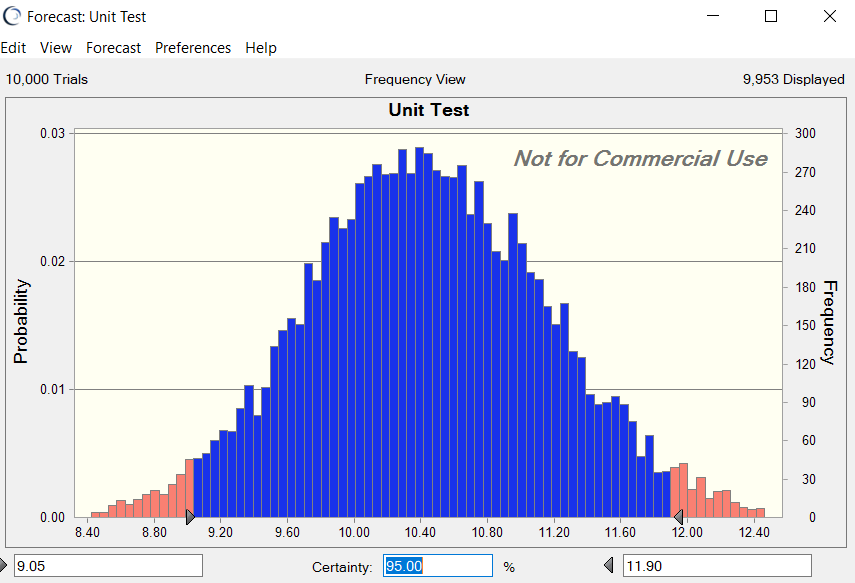
\includegraphics[width=6cm]{YH-UT.PNG}

\begin{itemize}
\tightlist
\item
  如果我们把优化后的缺陷分布(右图)与本来迭代的缺陷分布(左图)比较,能看出改进后,本来在系统测试才发现的缺陷大多数可以预先在评审暴露,降低返工工作量,也可以预估评审缺陷范围,如果实际评审缺陷数未能达到范围,便可预警,尽快纠正。
\end{itemize}

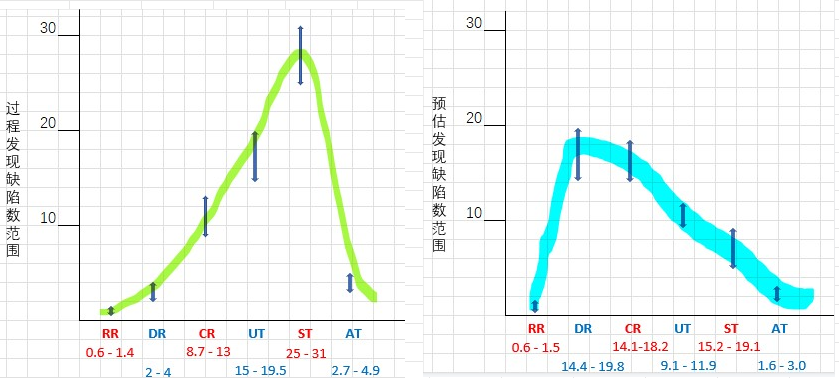
\includegraphics[width=6cm]{MTKL.png}

如果没有预测模型,我们只能主观估计会降低,有了预测模型,便可以估计缺陷分布的变化,也能帮我们挑选最佳搭配,并预估下一轮的缺陷分布范围。

\textbf{解读预测模型最佳搭配选择:}\\
模型以总成本最低可以防止局部最优。例如,需求评审没有选用排除率高的新方法,因为新方法会使用较大评审工作量。如果用质量最优(质量成本最低)便必然会读选用缺陷排除率最高的方法,但用总成本来比较便可以综合考虑工作量(Effort)
和 质量(Quality),避免局部最优。

今次有3种新方法比较,共8个配搭。假如3类评审都有两种新方法可选,我们便要比较
27 (3 x 3 x
3)配搭,每个配搭都单独模拟预估成本,然后统一比较,会非常费时,水晶球的最优功能能帮助快速选出最佳配搭。

质量经理:做了第一轮迭代后,以后的迭代有什么要注意?\\
我:团队累积了多轮迭代数据,便可以开始分析数据,并开始建立标杆。\\

\hypertarget{ux5efaux7acbux56e2ux961fux6807ux6746ux57faux7ebf}{%
\subsection{建立团队标杆(基线)}\label{ux5efaux7acbux56e2ux961fux6807ux6746ux57faux7ebf}}

第一轮做模型估算,有些新方法的参数,例如需求评审排除率,都是随便预估出来。但第二轮迭代回顾时,便有实际的数据依据来调整缺陷排除率,更新模型预测参数,使下一轮的预估缺陷范围更能反应实际、更准确。当团队一直每轮都是用这个方式去完善后,就可以建立团队标杆作参考。

例如代码评审的缺陷率,从以往迭代数据可以得出上下限范围判断新一轮迭代的缺陷率是否超出范围。关于如何利用迭代的数据,用控制图判断是否稳定建立上下限范围,会在控制图(25章)里详细说明。

\framebox{%
\begin{minipage}[t]{0.97\columnwidth}\raggedright
注意:上面我们是说缺陷率发现的缺陷数除以迭代的规模数,而不是说缺陷数,因为每次迭代的规模都不同,迭代的缺陷数是无法比较的,但是缺陷率就可以比较了。所以利用简化功能点估算规模是团队量化管理的基础。
\strut
\end{minipage}}

\hypertarget{ux4eceux8fedux4ee3ux590dux76d8ux5230ux6301ux7eedux6539ux8fdb}{%
\subsection{从迭代复盘到持续改进}\label{ux4eceux8fedux4ee3ux590dux76d8ux5230ux6301ux7eedux6539ux8fdb}}

回顾时做好复盘根因分析,利用数据,改善下一轮开发质量。
如何可以变成团队或公司的持续改进呢?

\framebox{%
\begin{minipage}[t]{0.97\columnwidth}\raggedright
深圳有一家公司专门是做内部IT服务。因为要求很严格,都要经过测试验收都通过,才允许新版本正式投产(发版)。每两周会做一次发版,每次都会统计发版成功率,因为都做了很久,依据以往水平,要求发版成功率不会低于96\%,并一直都监控这个百分比趋势。某一个月发现成功率跌到接近96\%。质量改进组就开始启动根因分析。先看是哪个部门出问题引起发板率低。发现有两个部门表现最差,然后针对这两部门做根因分析找出具体原因。然后也对应一些原因做了纠正措施,比如培训评审等等,做以后发现确实那些问题解决了。发版率的水平也提升了,后面他反而可以把那个变成新的基线,变成一个新的水平。到了98\%,
\strut
\end{minipage}}

从以上例子看到,按成功率,或缺陷率,从趋势,制定标杆,使用根因分析,针对根因采取纠正措施,质量提升,升到一个新的水平。


\hypertarget{ux7ed3ux675fux8bed}{%
\subsection{促进公司过程改进}\label{ux7ed3ux675fux8bed}}

做好根因分析,不仅仅能帮助团队提升,也可以帮助公司加强部门之间的沟通,帮助大家改进、提升。

我本来想问某家专注医院系统产品公司的质量经理,是否有很多缺陷在后期暴露,希望把缺陷前移,减少返工。他觉得这不是他们问题的重点。 

\framebox{%
\begin{minipage}[t]{0.97\columnwidth}\raggedright
他举例:“很多需求只是简单写一句话,所以不仅仅是开发与编码的问题。我们的产品经理都没有做什么过滤分析,直接把客户的简单需求发给开发,导致后面缺陷很多,客户验收时才发现问题。”

然后他打开系统说,“例如,这条需求只是简单一句话写了客户需要简化外科医生的流程,有些审批步骤可以简化。但需求人员没有详细写清整个流程与步骤,整个流程跟相关的页面有什么特殊处理。可以想象,开发人员还是会一头雾水,做出来肯定不能满足客户要求。 "
\strut
\end{minipage}}

为了促进部门之间沟通,我们组织了两天互动工作坊培训,主题是:“X通XX 2024:提升客户体验,实现价值交付",邀请了产品经理、项目经理、研发、设计、测试和实施/交付等都参加,分成四组,每组 8到10人。

第一天早上,先用机场数据学习怎么利用KJ分析方法和帕累托图,让大家开始利用数据分析根因。下午,小组按自己的角色列出满意和不满意的实例,并预计一年后的理想场景,提升大家兴趣与动力,因为如果只讨论解决问题,参与者反而会没有动力。最后引入度量与分析的主要概念,如 SMART 原则,定目标。利用GQM概念(详见附件)收集一些能帮助分析的数据,而不是什么数据都收集。大家按希望的场景列出具体的量化目标。

第二天,分组依据模拟缺陷数据分析根因,并利用水晶球模型预测下轮迭代效果。 


我发现某些组提出的改进建议是超出团队自己可以改进的范围,便说:

过程改进不仅仅是团队提升,也需要公司级配合才有效。如何可以做到公司级提升?例如某些团队需要公司级做好新员工培训,就需要成立过程改进小组,过程改进小组,通常会按功能分工。和你们按分功能分组一样,有专门需求或产品经理的小组、专门做研发的小组、针对设计的小组等,每个过程领域都应该有相关的改进小组专门探索有哪些地方可以改进,如何改进。 


所以我们下午就按这个思路要求每个团队写出希望改进的重点。然后让大家回顾,两轮讨论后,最终形成大家都接受并赞同的改进点和对应的改进行动:短期三个月,和长期行动计划(例如一年)。最终形成一份团体报告,向高层汇报。

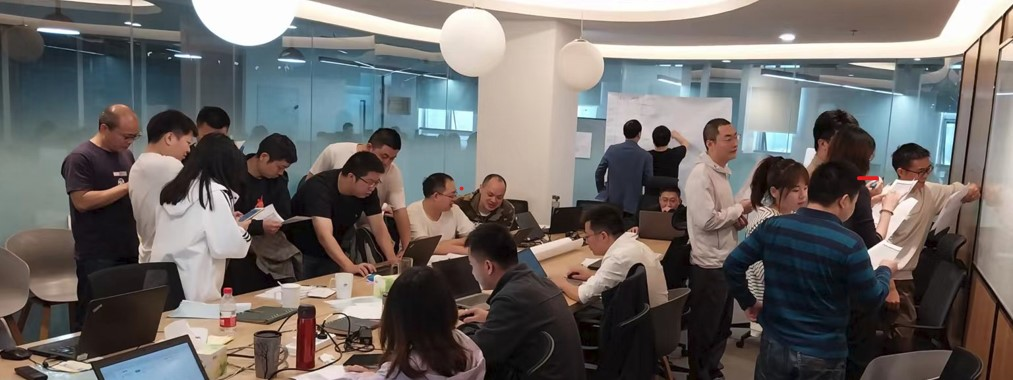
\includegraphics[width=6cm]{cdWS2Screenshot_2023-10-31_144622.jpg}

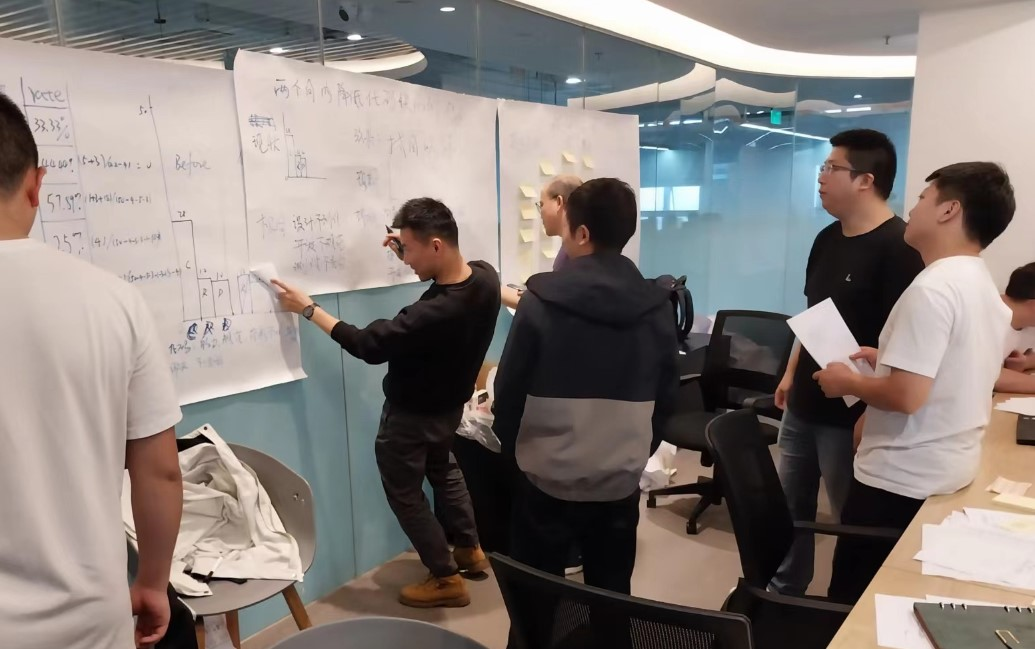
\includegraphics[width=6cm]{cdWS1Screenshot_2023-10-31_144121.jpg}


虽然公司的问题不仅仅是要缺陷前移,但还是可以利用缺陷前移根因分析,带出迭代回顾的重要性和量化管理,加强部门之间的交流沟通。例如:

产品经理能了解到研发人员的困难:研发代表:“今天早上有个紧急需求,下午五点钟前就要交付。”

"需求人员也听得到交付人员的困难:“医院客户要求很高,但因为有些实施人员工程师经验不足,延误了整个部署,导致客户不满。”

以两天工作坊培开始,再配合高层定期监控(例如改进小组每季度汇报),就可以帮公司建立持续改进的文化,加强了部门之间的正面沟通。


某项目经理参加了两天的培训后说,“虽然我们一直都有定期部门会议,但没有机会像这两天这样大家聚在一起讨论并了解,今次确实听到很多其他的部门的声音,让我们可以更全面了解到问题所在,这种沟通也能帮助大家互相协调,不会仅仅是把困难放在自己心里,但却无法解决。” 


\framebox{%
\begin{minipage}[t]{0.97\columnwidth}\raggedright
注意:在这种场景,老师(或内部教练)的任务是鼓励各人“发声”,自由发表自己的意见,反应事实,所以培训开始时要强调以下原则:

    1.让各岗位成员一起寻找改进方案。\\
    2.看全局,大家一起寻找共同点(避免瞎子摸象)。\\

强调从以前传统的依靠顾问专家指导思维,变为第2章提过的“所有员工参与改进整个系统”。

%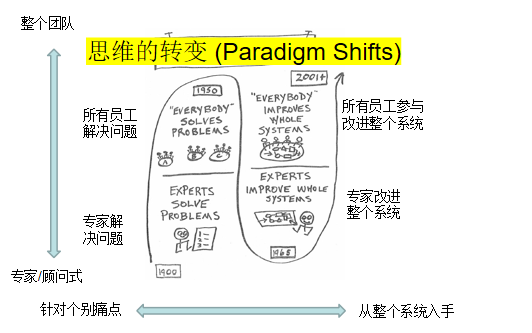
\includegraphics[width=6cm]{微信截图_20231025084623.png}

所以老师不要希望在工作坊里“教”大家,使他们提升,而是大家自己通过沟通交流,发现共同点,制定改进行动。

我五年前帮另一家北京公司做工作坊互动培训时,尝试教团队如何做好根因分析,引导他们基于公司目标选择自己的度量项等。虽然最后小组还是按我的意思去写了总结报告,展示高层。但培训后果就没有下文了,所以重点不是学员学到什么新的方法,最重要让他们动起来,自己动脑筋自己发现有那些方面立马可以做改进,他们才有动力后面执行,所以应尽量减少干涉,只是要求他们按时间完成指定任务,具体什么根因,什么改进方法让他们自己想,过程中也可利用功能性分组帮助团队成长(参考附件实例)。 

\strut
\end{minipage}}

\hypertarget{ux7ed3ux675fux8bed}{%
\subsection{结束语}\label{ux7ed3ux675fux8bed}}

Kent BECK
先生的极限编程,快速迭代,每一轮交付对客户有价值的产出物,并得到客户反馈,而不是花精力写文档(如,设计文档)。如能做好每次迭代回顾,便可以持续改善(类似丰田方式)。

要推动公司团队做好迭代回顾,必须先获取高层的认同与支持。

\framebox{%
\begin{minipage}[t]{0.97\columnwidth}\raggedright
为了引发领导兴趣,我先问三个问题:

\begin{enumerate}
\tightlist
\item
  你们觉得占工作量最多的是哪一类工作?
\item
  你们现在的缺陷绝大部分是在什么过程暴露?
\item
  你们估计验收/系统测试缺陷的返工工作量是多少?
\end{enumerate}


接下来,我就按“11 如何降低软件开发质量成本”讲,很多人低估了缺陷返工所耗费的工时,导致大部分的工作量都用于修复后期验收/系统测试的缺陷,软件开发的特性是缺陷越后期发现,返工工作量越高,如果每次迭代能把后面才发现的缺陷预先在前面发现并解决,不仅仅提高质量. 同时因减小后面的大量返工,同时也提高团队生产率。

这方法可以有效地在头15分钟让管理层/开发组长体会到针对缺陷前移做好根因分析的好处。
\\strut
\end{minipage}}



有了管理者的关注与支持,要做好迭代回顾,必须所有团队成员都参与,并赋予团队充分时间分析、讨论改进行动。

要基于数据做好回顾分析,最困难不是数据分析,而是怎么收集到真实的数据。所以必须在培训里,让学员知道为什么要收集数据,为迭代收集数据做好准备。

如果希望干系人有执行改进行动的动力,必须要他们在回顾时全心投入参与讨论,一起找根本原因和解决方案。所以培训时,不仅仅是教分析的技巧,更需要多利用互动游戏让他们可以放心发表意见。避免迭代回顾时,项目经理`一言堂'。

当数据不是单点而是分布时,蒙特卡罗预测模型可以帮我们更好处理数据。针对如何把发现缺陷前移,模型可以从每个过程的分布预估总返工工作量成本分布,也可以比较不同的搭配,自动挑选哪个搭配的总成本最低。

分析方法和可以改进的方向很多,这部分主要以一些实例带出每一个步骤的重点。大家掌握了这些节奏之后,就可以融会贯通,持续进行根本原因分析,形成不断优化的良性循环。以提升质量为目标,不再习惯于当前的缺陷水平,觉得大量缺陷在后期测试时被发现是正常。

%请不要误以为这部分提到的方法,工具是做好团队回顾的唯一方法。因大部分团队都有这问题,缺陷相关数据也比较容易收集到,所以建议先从缺陷前移入手,容易快速看到效果。分析缺陷排除根因取得效果后,可以继续探索其他改进方向,例如除了硬数据(缺陷数,工作量等),也可分析软数据(团员的心情,部门间的合作性等)。方法、工具会不断有新的取代,利用数据,分析根因,希望避免同类问题再发生,持续改进这些原则才是做好迭代回顾的重点。

\hypertarget{ux4e0dux4ec5ux4ec5ux9002ux7528ux4e8eux5206ux6790ux8fedux4ee3ux7f3aux9677ux6570ux636e}{%
\subsection{不仅仅适用于分析迭代缺陷数据}\label{ux4e0dux4ec5ux4ec5ux9002ux7528ux4e8eux5206ux6790ux8fedux4ee3ux7f3aux9677ux6570ux636e}}

请不要误以为这部分提到的方法、工具是做好团队回顾的唯一方法。因大部分团队都有这问题,缺陷相关数据也比较容易收集到,所以建议先从缺陷前移入手,容易快速看到效果。分析缺陷排除根因取得效果后,可以继续探索其他改进方向,例如除了硬数据(缺陷数,工作量等),也可分析软数据(团员的心情,部门间的合作性等)。方法、工具会不断有新的取代,利用数据,分析根因,希望避免同类问题再发生,持续改进这些原则才是做好迭代回顾的重点。

\hypertarget{ux9a71ux52a8ux6574ux4e2aux516cux53f8ux7684ux8fc7ux7a0bux6539ux8fdb}{%
\subsubsection{驱动整个公司的过程改进}\label{ux9a71ux52a8ux6574ux4e2aux516cux53f8ux7684ux8fc7ux7a0bux6539ux8fdb}}

分析缺陷排除率,做好根因分析,降低后期的缺陷密度,不仅仅对团队的提升有作用,也可以帮助整个公司,加强部门之间的沟通,帮助大家改进、提升。

例如某家专门是做医院系统产品的公司。我本来想问他是否希望很多缺陷在后期暴露,希望把缺陷前移。他听完以后,觉得这不是公司的问题重点。



\framebox{%
\begin{minipage}[t]{0.97\columnwidth}\raggedright
他举例,“很多需求只是简单写一句话,所以不仅仅是开发与编码的问题。我们的产品经理都没有做什么过滤分析,直接把客户的简单需求发给开发,导致后面缺陷很多,客户验收时才发现问题。

然后他打开系统(他们的缺陷都在系统管理),例如,有一条需求只是简单一句话写了客户需要外科医生的一个流程的简化。有些审批步骤可以简化,但需求人员没有详细写明整个步骤如何,整个流程跟相关的页面有什么特殊处理,可以想象,这种的话扔到开发还是一头雾水,肯定做出来的不能达到客户要求。"
\strut
\end{minipage}}

为了解决这个部门之间沟通,我们的组织了两天互动工作坊培训,主题是《X通XX
2024:提升客户体验,实现价值交付》,邀请了产品经理组商务经理组研发设计测试,和实施交付等都参加,分成四组,每一组8到10人。

第一天,早上先用机场数据要他们用KJ分析方式和帕累托图开始学习,怎么利用数据分析根因。下午就是让每个小组按自己的角色列出他满意和不满意的点。并预计一年后到2024年底理想的状态,因为如果只是谈解决什么问题,反而参与者会没有动力。如果先采用一些希望的未来场景,他们就有动力,更积极参与。最后用一有多小时开始引入度量与分析的主要概念,如
SMART
原则,定目标。利用GQM概念收集一些能帮助分析的数据,而不是什么都收集。要他们按希望的场景列出具体的量化目标。

第二天,我们利用水晶球模拟数据,要求每一组用半天时间就缺陷排除率的根因分析,并利用水晶球模型预测下轮迭代效果。过程里,组里成员就提出一些改进建议,是超出团队自己可以改进的范围。

\framebox{%
\begin{minipage}[t]{0.97\columnwidth}\raggedright
我便趁这个机会总结给团队说:\\过程改进,其实不仅仅是团队个别的提升,也需要整个公司级配合才更全面。如何可以做到公司级的提升。比如有些需要公司级做好新员工的培训等,这就需要成立过程改进小组,过程改进小组,通常会按功能分。正如你们现在分功能一样,有专门是需求或者产品经理的团队,专门做研发的团队,专门做设计等,每个过程领域都应该有相关的改进小组专门探索有哪些地方可以改进,如何改进。
\strut
\end{minipage}}

所以我们下午就按这个思路要求每个团队写出希望改进的重点。然后让大家回顾,两轮讨论后,最终形成大家都接受并赞同的改进点和对应的改进行动:短期三个月,和长期行动计划(例如一年)。最终形成一份团体报告,向高层汇报。

虽然公司的问题不仅仅是要缺陷前移,但还是可以利用缺陷前移根因分析,带出迭代回顾的重要性和量化管理,大家都就可以加强部门之间的交流沟通。

*产品经理能了解到研发人员的困难:研发代表:“今天早上有个紧急需求,下午五点钟前就要交付。”

"需求人员也听得到交付人员的困难:“医院客户要求很高,但因为有些实施人员工程师经验不足,延误了整个部署,导致客户不满。”

以两天工作坊培开始,再配合高层定期监控(例如改进小组每季度汇报),就可以帮公司建立持续改进的文化,加强了部门之间的正面沟通。

某项目经理参加了两天的培训后说,``虽然我们一直都有定期部门会议,但没有机会像这两天这样大家聚在一起讨论并了解,今次确实听到很多其他的部门的声音,让我们可以更全面了解到问题所在,这种沟通也能帮助大家互相协调,不会仅仅是把困难放在自己心里,但却无法解决。''

\framebox{%
\begin{minipage}[t]{0.97\columnwidth}\raggedright
注意:在这种场景,老师,或内部教练,的任务是鼓励各人``发声'',自由发布自己的意见,反应事实,所以培训开始时要强调这原则,也可参考附件:功能性分组帮助团队成长实例。

%\url{文件:johnWeirScreenshot2023-10-20134410.jpg}

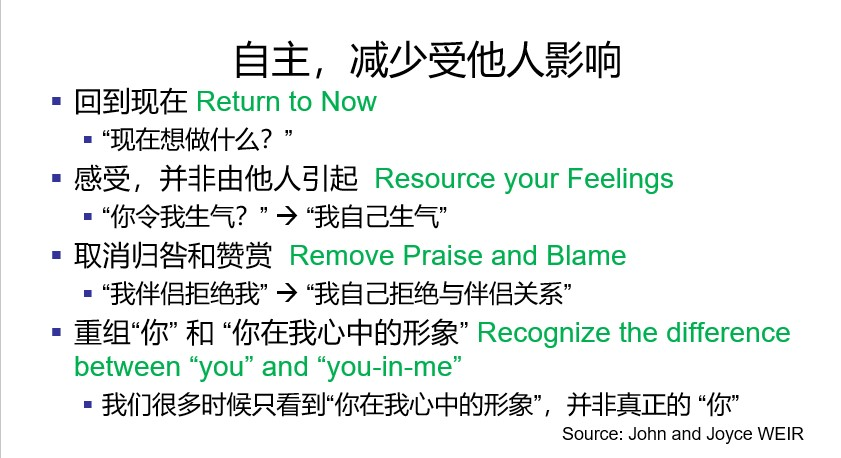
\includegraphics[width=6cm]{johnWeirScreenshot2023-10-20134410.jpg}

\strut
\end{minipage}}


\framebox{%
\begin{minipage}[t]{0.97\columnwidth}\raggedright
如何做好迭代回顾:'''总结'''

有数据才可以谈改进,有数据支撑的根因分析可以帮我们在下一个迭代做改进。因为改进花精力,所以必须有针对性,二八原则可以帮助识别应针对哪方面入手。软件开发应,软件开发团队花最多工作量的不是编码本身,用于修复缺陷工作量最多。软件开发有个特点,缺陷越后暴露,返工工作量越多,例如如果缺陷在客户使用后才暴露,可能总共要花30 - 50人时修正,但如果缺陷能在前面评审或单元测试发现和改正,就不会超过1人时。但如果回看每次开发交付,分析缺陷分布,大部分缺陷都是在系统测试或验收时才暴露,前面评审、单元测试、集成测试发现的缺陷都很少。


如果团队可以提前在评审、单元集成测试预先发现缺陷,不仅仅能提升产品的质量,让客户更满意,也可以节省团队工作量,提高生产率。

如果团队能在迭代复盘时或者迭代回顾时,一起分析缺陷排除率,针对占比最多的种类,使用便利贴方式KJ方式一起分析根因,制定下一轮的纠正措施,便可以把缺陷发现时间前移。


虽然很多团队的根因分析用了帕里拖图、鱼骨图的方式,这些都是基于主观判断的方式,没有真正利用基于事实的数据,而且很容易受从众心理影响,变成项目经理的一言堂,无法挖掘出真正原因,使用便利贴KJ方式可以帮团队,更好从事实总结出背后的主因。团队所有成员一起,包括需求、开发、测试、项目经理等一起分析迭代的缺陷数据,可以计算迭代的缺陷注入和缺陷排除率,利用蒙地卡罗预测模型就可以把本来只是定性的一个改进目标变成定量。

例如,如果需求评审的缺陷数未达到本来预计的范围,就可以预警团队可能评审力度还不够,没有得到效果,很可能不少缺陷,还是会等到后期才暴露,就可以立马加强力度,提高本迭代质量提升的概率。

根因分析不仅仅能改善团队产品质量问题,也可以用于其他改进,如用于两天的工作坊互动培训中,加强公司功能部门之间的协调,配合公司发展目标,相关过程改进小组制定短期和长期改进量化目标,帮公司过程改进升一台阶。

\strut
\end{minipage}}

\framebox{%
\begin{minipage}[t]{0.97\columnwidth}\raggedright
乔布斯,当NEXT CEO 时,被访问,谈质量:

整个质量提升的道理其实很简单,是一个重复的过程,然后我们需要不断去看,有哪些无效的环节要省略,哪部分要重新设计,不断试验、提升,就这么简单。重点是所有的提升都应该是科学化的,有数据而不是泛泛而谈。

\strut
\end{minipage}}

极限编程(XP)的最佳实践可帮我们发现现在的开发过程有那些不足,也有助找出具体根因和纠正措施,下一部分会探索里面的实践能如何帮助团队提升软件开发质量。


\hypertarget{ux9644ux4ef6}{%
\section{附件}\label{ux9644ux4ef6}}

\hypertarget{fmea-ux5b9eux4f8b}{%
\subsection{FMEA 实例}\label{fmea-ux5b9eux4f8b}}

\begin{description}
\tightlist
\item[]
(FMEA: Failure Mode Effects Analysis)
\end{description}

大家可能都遭遇过由于没有管理好时间,而导致迟到的情况.以坐飞机为例,从离开酒店到登上飞机的过程中,很可能因为一些风险导致最后没搭上飞机。\\
你出发的时候,可能用不同的交通方式:出租车、机场大巴等。如果你不能在起飞前45分钟到达机场办理登机牌,你便搭不上飞机。但是你拿了登机牌也有可能最后搭不上,因为飞机都严格执行起飞前15分钟关舱门所以你拿了登机牌,还要在起飞前
15 分钟到达登机口。

Fig 1 登机过程

%\url{文件:风险与机会1.png}

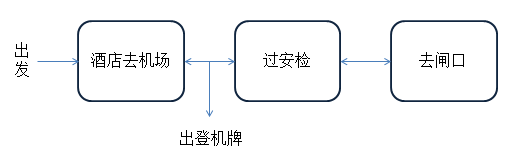
\includegraphics[width=6cm]{风险与机会1.png}


要赶上飞机其实是个过程,中间有很多环节会导致最后失败,所以我们可以通过FMEA过程分析来看如何减少失败的概率。

Fig 2 FMEA 例子

%\href{文件:风险与机会2_FMEA.png}{文件:风险与机会2 FMEA.png}

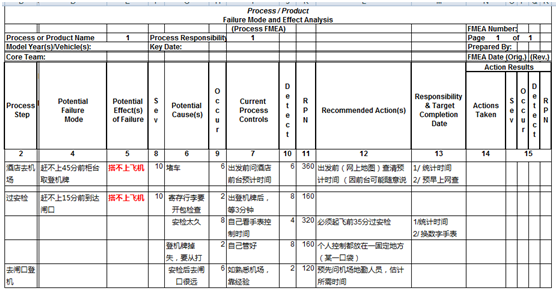
\includegraphics[width=6cm]{风险与机会2_FMEA.png}

Fig 3 打分参考

%\href{文件:风险与机会3_打分参考_1.png}{文件:风险与机会3 打分参考 1.png}

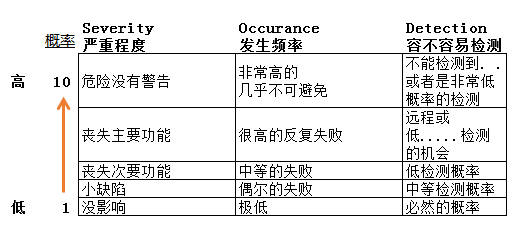
\includegraphics[width=6cm]{风险与机会3_打分参考_1.png}

以第一个失效为例:如发生便坐不上飞机,所以严重性是最高10。发生的概率还是比较高6。是否容易预防、预警。因不熟悉当地情况,加上我主要靠问酒店前台,有时候她也不清楚,所以我定6。
RPN = 10x6x6=360。

从以上登机的例子可以看出FMEA是以整个过程来管理风险,比如在出发前,就要查询一下各个交通工具要花费的时间,比如你发现在南京,从酒店坐地铁要转车,要花1个小时以上,如果时间太紧就来不及,宁可多花钱打车,才能控制风险。
当你拿了登机牌,还是要经过安检,还要从安检走过登机口。有时候机场很大,到达登机口也要花很长时间,就要先问好路径,提前计算好时间,才不会误点。\\
过了安检到登机口要10分钟以上,就要在起飞前的35分钟完成通过安检,才来得及。这些都可以通过FMEA的形式把整个坐飞机的过程识别出来,找各个阶段会出现的问题,就知道如何控制。

以这坐飞机的风险为例,我自己就多次未赶上飞机,原因很多,但总结一下都是习惯没改过来。我应依据以往差点赶不上的经验,回顾一下,确保每一个过程都控制住,就不会后面再次出问题
,这个和企业做风险管理概念一样。\\
有度量才有管理。人和公司一样,很多做的事情好像是自己主动去想,其实很多都是潜意识习惯,如果你没有定一些量化的控制手段,就不会提高这方面风险意识,还是会搭不上飞机。我先回顾以往几次搭飞机的情况,并把每次到达机场的时间和到达闸口的时间写下(详见下面
Fig 4 )\\
Fig 4 上面是机场柜台关闭(45分钟)前到达时间,下面是关闸口前到达时间
(分钟)( X 代表赶不上飞机)

%\url{文件:风险与机会4.png}

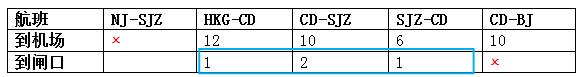
\includegraphics[width=6cm]{风险与机会41.png}

最近一次赶不上飞机是因为未能在关闸门前到,之前已发生过两次 -\/-\/-
我刚到闸口,就到时间马上关闸了 !\\
如果我把经验教训记下来,下次做好时间管理,就会避免后面的延误:有了数据,我们便可以更有效在回顾时做好根因分析
(CAR)。\\
以这登记延误风险为例,可以使用FMEA分析每一失效点,例如过安检(因没有预留足够时间)与从安检到闸口太长时间等的发生概率都很高
(前者8, 后者 6)\\
为了避免问题再发生,就要定一些具体的计划,最终希望把误点减到零。\\
在登机这个环节,可利用什么有效方法/工具,帮助改善?

-
每次出发去机场前都查询各种交通方式的时间与风险(概率),预留足够时间,降低失效发生的概率\\
- 拿了登记牌后,都计划好必须起飞前35分通过安检,45分前开始安检

在多次没登上飞机后,我发现平常的手表没有正负5分钟的概念,但是如果用电子手表,对时间的感觉可以准确到了正负1分钟,就能够更好把控时间。

Fig 5 平常用于培训 / 评估计时的电子钟

%\href{文件:风险与机会5_闹钟.png}{文件:风险与机会5 闹钟.png}

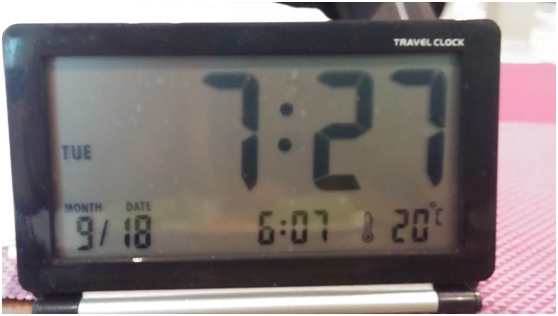
\includegraphics[width=6cm]{风险与机会5_闹钟.png}

经过这次误机,我就买了个电子手表,取代传统针式手表,希望对日后不迟到有帮助。

\textbf{效果}: 这故事发生在2019.9
,后面我按这些计划,一直都没有再出现赶不上飞机的情况,我每次都提醒自己必须在起飞前60
\textasciitilde{} 90分钟到机场,30 \textasciitilde{}
45分钟前到闸口。分析的目的是提高个人风险意识,避免问题发生。

\hypertarget{ux529fux80fdux6027ux5206ux7ec4ux5e2eux52a9ux56e2ux961fux6210ux957fux5b9eux4f8b}{%
\subsection{功能性分组帮助团队成长实例}\label{ux529fux80fdux6027ux5206ux7ec4ux5e2eux52a9ux56e2ux961fux6210ux957fux5b9eux4f8b}}

系统,包括团队、公司,的成长都依靠不断集合内部的差异,如果完全不能接受不同意见,就无法进步。基于心理学家
Yvonne Agazarian 系统中心理论 (Systems Centered
Theory),团队必须先从成见分组(Stereotype subgroup)
变为功能性分组(Functional Subgroup),才能成长。

要让大家觉得有共同点。基于这基础才可以听从不同意见。但首先要让大家愿意接受不同意见,不然的话就会变成争吵,不会有效果。
有人提出不同意见后,必须有人附和,成为他的战友,才能形成新的小组。有了新小组以后,团队需要把不同小组的立场合并起来,变成一个新方向、新思路,整个团队就有成长、进步。

\framebox{%
\begin{minipage}[t]{0.97\columnwidth}\raggedright
 场景实例:\\团队讨论如何完善社区里面的教育,大家讨论个人的希望。\\ 
A:好像我们大家的想法都很类似。\\ 
内部教练:可否举个例子?\\ 
B:我们都想为自己和我们后代有个终身不断学习的机会。\\
C:好像我们都没有人提过大学,不知道为什么。\\
 D:但很多人负担不起大学学费。\\
 E:我觉得每个人只要想受到教育,都能做到,我就是靠自身努力。最后完成大学教育。\\
 F:(开始跟D形成小组)是的,但教育确实越来越昂贵,
我估计我们当中不少人负担不起那些美国东岸名校的昂贵学费。\\ 
G:(有成见,觉得那些不能完成大学教育的都是没有动力,没有上进心)我还是觉得任何人,只要有动力都能做到。\\
 如果没有人附和E的观点,就可能变成他的个人独角戏。后面有两个可能的发展场景:\\
 场景一C 附和了E的观点。\\ 
C:我的经历确实和E说的类似,辛辛苦苦最终完成了大学教育,但确实很艰苦。
如果我当时没有舅舅的支持,肯定完成不了。\\ 
场景二 没有人附和E的说法。\\ 内部教练:有没有其他人也有经过自己努力完成大学教育的经历?\\ (注意:内部教练千万不能说:``有没有人赞同,人只要有动力都能进大学?''因为这只是个人观点,并非事实。)\\
 A:我确实也完成了大学教育了,但也经历了很多困难。\\
 G:我读了一年,因为再得不到奖学金,没有办法,只能退学。\\
到了这个点,整个分组就比较复杂,虽然生成了新小组,
E得到一些回应,但也有些人提出不同的经验,需要有说法把新小组归纳。\\
 接下来,\\
 C:我看来这个很简单,有些人能完成大学教育。有些人虽然很希望完成,最终还是完成不了,但不是所有人都想或者必须完成大学教育。所以我们的改进任务应该是帮助所有人学到他希望学习的东西。\\
 有了以上C的说法,整个团队就可以进一步成长。

\strut
\end{minipage}}


\hypertarget{gqm}{%
\subsection{GQM}\label{gqm}}

\begin{description}
\tightlist
\item[]
G:Goal (目标)

Q:Question (问题)

M:Metric (度量)
\end{description}

收集数据很花精力,所以必须只收集与改进目标相关的数据,但如何能联想到那些度量使相关?GQM利用问题让我们找到相关的度量。

1.制定目标。

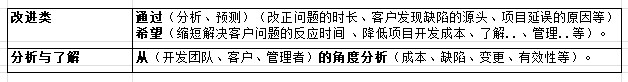
\includegraphics[width=6cm]{Gqm1Screenshot_2023-11-01_113815.jpg}

2.针对目标提出问题。

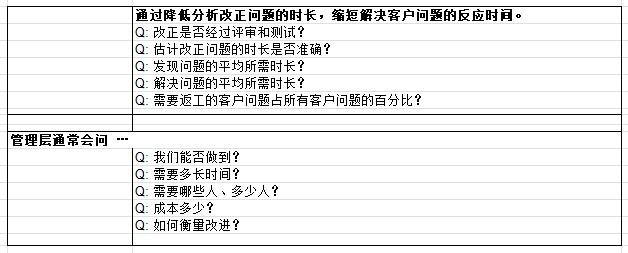
\includegraphics[width=6cm]{Gqm2Screenshot_2023-11-01_114014.jpg}

3.针对问题选择度量项。

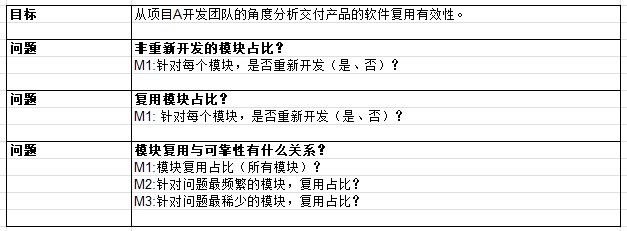
\includegraphics[width=6cm]{Gqm3Screenshot_2023-11-01_114048.jpg}

4.如何收集数据。

\begin{itemize}
\tightlist
\item
  谁来收集?
\item
  什么时候收集?
\item
  如何能有效收集数据并也保证正确?
\item
  谁是数据分析的对象?
\end{itemize}

5.收集、确认和分析数据,并反馈,让项目组制定纠正措施。

6.改进后分析数据,判断达标的程度。

7.做反馈,让所有利益相关者讨论。

有了目标与度量项,我们便可以制定度量计划。

%\href{文件:13_MA_plan_Screenshot_2023-10-26_211815.jpg}{650px}

%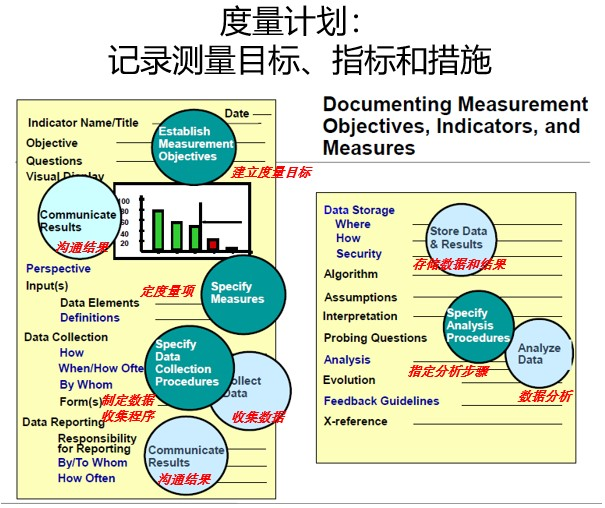
\includegraphics[width=6cm]{13_MA_plan_Screenshot_2023-10-26_211815.jpg}


\hypertarget{ux9644ux4ef6}{%
\section{参考 References}\label{ux9644ux4ef6}}

1. WEISBORD, Marvin: FUTURE SEARCH: Getting the whole system in the Room
for Vision, Commitment, and Action (2010 3/e)\\



